% Created 2009-12-16 Wed 10:59
\documentclass[11pt]{article}
\usepackage[utf8]{inputenc}
\usepackage[T1]{fontenc}
\usepackage{graphicx}
\usepackage{longtable}
\usepackage{soul}
\usepackage{hyperref}
\usepackage{color}
\usepackage{tikz}
\usepackage{listings}
\usepackage{movie15}
\hypersetup{
colorlinks=true,
linkcolor=blue,
citecolor=blue,
filecolor=blue,
urlcolor=blue,
pdfborder={0 0 0 0}
}

\title{Genetic Programming on IXM}
\author{Eric Schulte}
\date{16 December 2009}

\begin{document}

\maketitle


\definecolor{strings}{RGB}{60,179,113}
\lstset{
  keywordstyle=\color{blue},
  commentstyle=\color{red},
  stringstyle=\color{strings}
}
\hypersetup{
  linkcolor=blue,
  pdfborder={0 0 0 0}
}

\section*{Report}
\label{sec-1}

\subsection*{Introduction}
\label{sec-1.1}

A system of subpopulation Genetic Programming (GP) is implemented over
Illuminato X Machina (IXM)\footnote{\href{http://illuminatolabs.com/IlluminatoHome.htm}{http://illuminatolabs.com/IlluminatoHome.htm} } boards.  The GP system is designed in
the spirit of the IXM boards and attempts to explore the
intuitions\footnote{\href{http://reproducibleresearch.net/index.php/Main_Page}{http://reproducibleresearch.net/index.php/Main\_Page} } which served as the impetus for the board's creation.
A series of experiments assess the effects of varying traditional GP
parameters, of applying coevolution and of various physical layouts on
the relative success of the GP.  The inherently redundant and
distributed nature of subpopulation GP is shown to be a natural fit
for the IXM environment and directions for future work are discussed.
In the spirit of Reproducible Research\footnote{\href{http://livingcomputation.com/rpc/}{http://livingcomputation.com/rpc/} }, all source code and
experimental data referenced in this work is made available to the
reader (see \hyperref[sec-1.8]{reproduction}) in the hopes of encouraging further work in
this area.

\subsection*{Illuminato X Machina -- telos and construction}
\label{sec-1.2}

An IXM$^{1}$ board is a small square board containing an atom
processor, memory, a button, led lights, hardware timers, a power rail
and four connectors arrayed around the perimeter of the board.
Although each board is in essence a small self-contained computer they
are intended to be used in groups.  When multiple boards are connected
through they communicate and share power with their neighbors through
their side connections.

\begin{figure}[htb]
\centering
\includegraphics[width=26em]{data/big-grid.png}
\caption{37 IXM boards in operation}
\end{figure}

One goal of the boards is to enable experimentation with software
developed under a new set of assumptions.  On a grid of IXM boards the
central single CPU, the shared memory and the global clock of a
traditional computer are relinquished in favor of a dynamic set of
loosely coupled peers, each equipped with its own personal clock
processor and memory.  In such an environment robustness of operation
is achieved through the abandonment of privileged points in space and
time and the duplication of functionality across a largely homogeneous
populations of peers.

This work attempts to manifest these themes in a GP implementation
which will run effectively in the IXM environment.

\subsection*{GP -- implementation and defense of deviations from the norm}
\label{sec-1.3}

In an effort to better align with the IXM platform the GP system
employed in this work differs from GP norms in a number of areas.
These deviations will be defended as they arise.  The source code for
the GP implementation described below can be found in
\href{file:///nfs/adaptive/eschulte/src/gp4ixm-report/src/evolve-sketch.pde}{evolve-sketch.pde} and \href{file:///nfs/adaptive/eschulte/src/gp4ixm-report/src/coevolve-sketch.pde}{coevolve-sketch.pde}.  Both files use the
\href{file:///nfs/adaptive/eschulte/src/gp4ixm-report/src/collector/}{collector/} IXM library for communicating results back to a central
source.

\subsubsection*{Representation and Fitness}
\label{sec-1.3.1}

This approach evolves individuals which are represented as variable
length strings of integers and arithmetic operators in Reverse Polish
Notation (RPN).  The individuals are evaluated by their ability to
match a ``target'' string also represented in RPN.  The simplicity of
the RPN stack machine facilitated quick development on the IXM boards.

\begin{figure}[htb]
\centering
\includegraphics[width=26em]{data/rpn-stack.png}
\caption{RPN stack machine}
\end{figure}



The only difference between the individual strings and the possible
goal strings is the inclusion of the `sine' operator in the goal
strings.  This unbalance encourages interesting behavior of the
evolving individuals as they tackle the difficult task of
approximating a trigonometric function using arithmetic operators --
in effect evolving towards a Taylor Series.

\subsubsection*{Genetic Operators}
\label{sec-1.3.2}

New individuals are generated in the following three manners.  In each
of the following when an individual is needed as an input to the
operation that individual is selected from the population through
using tournament selection.
\begin{description}
\item[injection] A new individual is created from whole cloth.  Each
     element in the individual's RPN string is selected at random from
     the set of all valid RPN characters.  This is the process used to
     generated an initial population immediately after board boot-up.
\lstset{language=c++}
\begin{lstlisting}
char possibilities[16] = BUILDING_BLOCKS;
ind.representation[0] = possibilities[random(15)];
for(int i=0; i < random(IND_SIZE); ++i) {
  ind.representation[i] = possibilities[random(15)];
  index = i;
}
\end{lstlisting}
\item[mutation] An modified copy is made of an existing individual.
     First an exact copy is made, then each step of the copies RPN
     string is mutated with a probability equal to $1/mutation\_prob$
     where $mutation\_prob$ is a parameter of the GP system.
\lstset{language=c++}
\begin{lstlisting}
char possibilities[16] = BUILDING_BLOCKS;
for(int i=0; i<size(); ++i)
  if(random(size()) == mutation_prob)
    representation[i] = possibilities[random(15)];
\end{lstlisting}
\item[crossover] Single point crossover is used to combine to existing
     individuals to generate a new individual.  First a crossover
     point is picked for each parent, then the first half from one
     parent is combined with the second half from the other parent as
     shown.
\lstset{language=c++}
\begin{lstlisting}
int mother_point = random(mother->size());
int father_point = random(father->size());
for(int i=0; i<mother_point; ++i) {
  child.representation[index] = mother->representation[i];
  ++index;
}
for(int i=father_point; i<father->size(); ++i) {
  if((index+1) >= (IND_SIZE - 1)) break;
  child.representation[index] = father->representation[i];
  ++index;
}
child.representation[index] = '\0';
\end{lstlisting}
\item[sharing] During sharing an individual is selected and is ``shared''
     with all of the IXM board's neighbors.
\end{description}

\subsubsection*{Population Operations -- avoiding privileged points}
\label{sec-1.3.3}

Up to this point the GP system we have introduced is largely standard
and should be unsurprising.  Where our system differs from traditional
GP is in the timing and distribution of operations on the population
of individuals.  Since one of our goals is uniformity in both space
and time we discard the notion of a fixed population cycle and instead
perform all GP operations at constant frequencies.  As such there are
no discrete ``stages'' or ``steps'' in our GP.

Using hardware timers included on the IXM boards we scheduler the
operations of mutation, injection, crossover, and sharing to recur at
fixed frequencies.  The frequency of these operations are parameters
of the GP system.  Whenever one of these operations returns a new
individual (e.g. the product of crossover, or an individual shared by
a neighbor board) the new individual is incorporated into the
population and the current worst individual is removed form the
population.  The only time an individual will be removed from the
population is when it is displaced in this manner.

Given the above setup all of the GP operations are constantly acting
on the population in a semi-stochastic interleaved manner.  No
randomness is explicitly added to the operation scheduling (although
this would be sympathetic with our themes) however as the boards
periodically become too busy pending GP operations are can be delayed
adding an element of randomness to the system.

\subsubsection*{Board Layout}
\label{sec-1.3.4}

The following illustrates the functional components of our GP
framework as implemented out on a single board.

\begin{figure}[htb]
\centering
\includegraphics[width=26em]{data/board-layout.png}
\caption{Layout of a single IXM board}
\end{figure}



\subsubsection*{Properties}
\label{sec-1.3.5}

The GP system as described has the following properties which are
desirable for the IXM environment.
\begin{itemize}
\item all boards are peers
\item any number of boards can be used effectively -- including a single
  board
\item increasing the number of boards increases the effectiveness of the
  GP system -- following some asymptotic curve
\item boards can be added to the GP system during execution and
  incorporated \emph{on the fly}
\item the system degrades gracefully as boards are removed from the system
\end{itemize}

\subsection*{Experimental Methodology}
\label{sec-1.4}

All experiments are run using the following methodology.  A laptop
side \href{http://www.ruby-lang.org/en/}{Ruby} script (either \href{file:///nfs/adaptive/eschulte/src/gp4ixm-report/src/experimenter.rb}{experimenter.rb} or \href{file:///nfs/adaptive/eschulte/src/gp4ixm-report/src/coexperimenter.rb}{coexperimenter.rb})
communicates with an attached group of IXM boards using the \href{http://github.com/mixonic/libixm}{libixm}
Ruby library and the \texttt{sfbprog} command distributed with the core IXM
software.  The Ruby scripts take a series of parameters and for each
combination they
\begin{enumerate}
\item input parameters to the boards
\item initiate board execution
\item collect and save raw data output by the boards
\item timeout overrunning experiments
\item repeat
\end{enumerate}

The experiments presented below had running times between 1 hour and
close to 30 hours.  The scripts are executed using the \href{http://www.gnu.org/software/screen/}{gnu screen}
program to allow persistent execution while the user is not logged
into the machine.

The boards report all results using the \href{file:///nfs/adaptive/eschulte/src/gp4ixm-report/src/collector/}{collector/} IXM library.  The
collector library allows each board in a group to report parameters
back to a central ``collector'' appending a ``path'' to the returned
results.  The path can be used to uniquely identify the board and
assign it coordinates in the 2D geometry of the board layout.

All graphs generated as part of this report used the collector output
as saved by the above Ruby scripts along with the \href{file:///nfs/adaptive/eschulte/src/gp4ixm-report/src/group.rb}{group.rb} and
\href{file:///nfs/adaptive/eschulte/src/gp4ixm-report/src/board.rb}{board.rb} scripts.  These scripts translated the raw data into 2D
information in a form suitable for input to \href{http://www.gnuplot.info/}{gnuplot}.

\subsection*{Results}
\label{sec-1.5}

\subsubsection*{GP Parameters}
\label{sec-1.5.1}

Initial experimentation was aimed at ensuring both that our GP system
was able to solve simple tasks and that both GP operations (`mutation'
and `crossover') improved GP performance.

These results were generated running \href{file:///nfs/adaptive/eschulte/src/gp4ixm-report/src/evolve-sketch.pde}{evolve-sketch.pde} on a single IXM
board.  Mutation and crossover frequencies of 10 milliseconds and 100
milliseconds (m.10, b.10, m.100, and b.100 respectively) were tested
resulting in the runtimes shown below.  Times shown are the average
time taken to generate an ideal individual over 5 runs.  The results
indicate that both mutation and crossover reduce the runtime required
for the GP to solve problems.  In addition it appears that crossover
is more effective against harder problems (e.g. ``xxx**xxxx***+'') while
mutation is more effective against simpler problems (e.g. ``7xxx**+'').



\begin{figure}[htb]
\centering
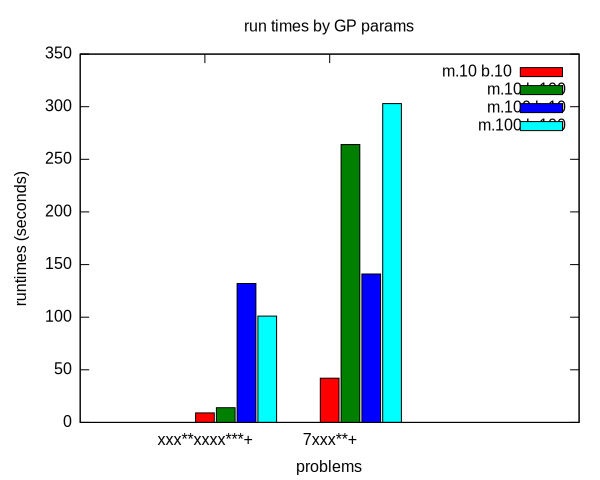
\includegraphics[width=26em]{graphs/gp-params.png}
\caption{runtime by GP parameters}
\end{figure}

\subsubsection*{Sub-populations and Sharing}
\label{sec-1.5.2}

After the basic GP operations had been verified we investigated the
effect of distributing the GP over multiple boards.  An series of runs
were performed using sharing frequencies of 100 milliseconds and
mutation and crossover frequencies of 10 milliseconds.  Times shown
are the average time taken to generate an ideal individual over 5
runs.  Although the effect of adding a second board was not dramatic
there is clear evidence that the addition of a second board and a
second population did increase the effectiveness of the GP.



\begin{figure}[htb]
\centering
\includegraphics[width=26em]{graphs/sharing.png}
\caption{sharing individuals across two boards}
\end{figure}

\subsubsection*{Sharing and Layout}
\label{sec-1.5.3}

Next the effects of different sharing rates run over a large group of
15 boards was investigated.  The sharing experiments were run over two
different board layouts -- a straight line and an altered figure
eight.  The results for each layout are presented as well as a
comparison between the two.  In all experiments below the following
three goals functions were used.  Each GP parameter combination was
allowed 10 minutes to attempt to fit each function.  10 runs were
performed in each setup and all reported results are the average of
the 10 runs.

\begin{figure}[htb]
\centering
\includegraphics[width=26em]{data/line.png}
\caption{line layout}
\end{figure}

\begin{figure}[htb]
\centering
\includegraphics[width=26em]{data/figure-eight.png}
\caption{figure eight layout}
\end{figure}

\begin{itemize}

\item line\\
\label{sec-1.5.3.1}

The runtimes for each sharing rate by goal.  All sharing rates are
reported in milliseconds.  In general the results seem to illustrate
the a sharing rate of 1000 milliseconds performs best.
\begin{itemize}

\item "xxx**xxxx***+"\\
\label{sec-1.5.3.1.1}


\begin{center}
\begin{tabular}{rr}
 sharing rate  &  ave. time to completion  \\
\hline
        10000  &                3.8355099  \\
         1000  &                3.2090558  \\
          100  &                3.2239733  \\
\end{tabular}
\end{center}




\item "7xxx**+"\\
\label{sec-1.5.3.1.2}


\begin{center}
\begin{tabular}{rr}
 sharing rate  &  ave. time to completion  \\
\hline
        10000  &                4.9986461  \\
         1000  &                3.1983512  \\
          100  &                2.1230925  \\
\end{tabular}
\end{center}




\item "xs55+55+**"\\
\label{sec-1.5.3.1.3}

This goal is equivalent to $100 sine(x)$ which is not possible for our
GP individuals to match as they do not have the sine function as one
of their operators.  The average best score for each sharing rate is
reported.

\begin{center}
\begin{tabular}{rr}
 sharing rate  &  ave. time to completion  \\
\hline
        10000  &                  invalid  \\
         1000  &                  156.743  \\
          100  &                  164.008  \\
\end{tabular}
\end{center}



the reason that the above results for 10000 are labeled ``invalid'' is
that is appears that some boards did not successfully have their goal
reset from ``7xxx**+'' to ``xs55+55+**'' in these runs, so no data is
available.

although no individuals exactly matched $100 sine(x)$ some did come
close, most notably the following whose RPN representation of
\texttt{x2*x6-/3x7+*x3x-*/+7*} expands to the following algebraic expression
\texttt{((((x * 2) / (x - 6)) + ((3 * (x + 7)) / (x * (3 - x)))) * 7)} which
does a very good job of matching the target function over the test
values of x with a best score of 136.07.



\begin{figure}[htb]
\centering
\includegraphics[width=26em]{graphs/evo_line_2_best.png}
\caption{best individual in range}
\end{figure}

although globally the fit is less impressive



\begin{figure}[htb]
\centering
\includegraphics[width=26em]{graphs/evo_line_2_best_wide.png}
\caption{best individual out of range}
\end{figure}

\end{itemize} % ends low level

\item figure eight\\
\label{sec-1.5.3.2}

The runtimes for each sharing rate by goal.  All sharing rates are
reported in milliseconds.  In general the results seem to illustrate
the a sharing rate of 1000 milliseconds performs best.
\begin{itemize}

\item "xxx**xxxx***+"\\
\label{sec-1.5.3.2.1}


\begin{center}
\begin{tabular}{rr}
 sharing rate  &  ave. time to completion  \\
\hline
        10000  &                3.6102906  \\
         1000  &                2.8806907  \\
          100  &                6.4068757  \\
\end{tabular}
\end{center}




\item "7xxx**+"\\
\label{sec-1.5.3.2.2}


\begin{center}
\begin{tabular}{rr}
 sharing rate  &  ave. time to completion  \\
\hline
        10000  &               24.0118271  \\
         1000  &                3.1030883  \\
          100  &                1.9693912  \\
\end{tabular}
\end{center}




\item "xs55+55+**"\\
\label{sec-1.5.3.2.3}

This goal is equivalent to $100 sine(x)$ which is not possible for our
GP individuals to match as they do not have the sine function as one
of their operators.  The average best score for each sharing rate is
reported.

\begin{center}
\begin{tabular}{rr}
 sharing rate  &  ave. time to completion  \\
\hline
        10000  &         255.311111111111  \\
         1000  &         183.966666666667  \\
          100  &         253.433333333333  \\
\end{tabular}
\end{center}



although no individuals exactly matched $100 sine(x)$ some did come
close, most notably the following whose RPN representation of
\texttt{0757x/3-x+3x-/**x/x+x*} expands to the following algebraic expression
\texttt{((((7 * (5 * ((((7 / x) - 3) + x) / (3 - x)))) / x) + x) * x)} which
does a very good job of matching the target function over the test
values of x with a score of 254.35.



\begin{figure}[htb]
\centering
\includegraphics[width=26em]{graphs/evo_eight_2_best.png}
\caption{best individual in range}
\end{figure}

although globally the fit is less impressive



\begin{figure}[htb]
\centering
\includegraphics[width=26em]{graphs/evo_eight_2_best_wide.png}
\caption{best individual out of range}
\end{figure}

\end{itemize} % ends low level

\item video results\\
\label{sec-1.5.3.3}

The following videos are provided to better illustrate the dynamic
fitness levels across multiple boards during the previous runs.  In
these videos each board is represented as a bar in a 3d histogram.
The placement of the bars mirrors the physical placement of the boards
and the height of the bar is equal to the most fit individual on the
board.  Recall that fitness is calculated as the \textbf{difference} between
an individual and the goal, so a lower fitness score is better.

\textbf{note}: If the following don't begin playing automatically they can be
download from \href{http://cs.unm.edu/~eschulte/classes/cs591-rpc/gp4ixm-report/videos}{here} and saved to your desktop.  On a mac you may need
to use \href{http://www.videolan.org/vlc/}{VLC} if your default video player doesn't understand these
files.

  \begin{figure}
  \centering
    \includemovie[poster, text={\small(videos/evo\_line\_100\_0\_0.mpg)}]{6cm}{6cm}{videos/evo_line_100_0_0.mpg}
  \caption{Formation: line Goal: "xxx**xxxx***+" Run: 0}
  \end{figure}


  \begin{figure}
  \centering
    \includemovie[poster, text={\small(videos/evo\_line\_100\_1\_1.mpg)}]{6cm}{6cm}{videos/evo_line_100_1_1.mpg}
  \caption{Formation: line Goal: "7xxx**+" Run: 1}
  \end{figure}


  \begin{figure}
  \centering
    \includemovie[poster, text={\small(videos/evo\_line\_100\_2\_1.mpg)}]{6cm}{6cm}{videos/evo_line_100_2_1.mpg}
  \caption{Formation: line Goal: "xs55+55+**" Run: 1}
  \end{figure}


  \begin{figure}
  \centering
    \includemovie[poster, text={\small(videos/evo\_eight\_100\_0\_1.mpg)}]{6cm}{6cm}{videos/evo_eight_100_0_1.mpg}
  \caption{Formation: eight Goal: "xxx**xxxx***+" Run: 1}
  \end{figure}


  \begin{figure}
  \centering
    \includemovie[poster, text={\small(videos/evo\_eight\_100\_1\_1.mpg)}]{6cm}{6cm}{videos/evo_eight_100_1_1.mpg}
  \caption{Formation: eight Goal: "7xxx**+" Run: 1}
  \end{figure}


  \begin{figure}
  \centering
    \includemovie[poster, text={\small(videos/evo\_eight\_100\_2\_1.mpg)}]{6cm}{6cm}{videos/evo_eight_100_2_1.mpg}
  \caption{Formation: eight Goal: "xs55+55+**" Run: 1}
  \end{figure}


\end{itemize} % ends low level
\subsubsection*{Coevolution}
\label{sec-1.5.4}

Coevolution was implemented by evolving a Genetic Algorithm (GA) over
the x values to be checked.  The coevolution task was significantly
more difficult than the related evolutionary task as a much wider
range of possible x values was used.  While all pure evolution
experiments were run over the static range of integers between 0 and
10 the coevolution x values ranged from -100 to 100.  Each x-range
coevolution ``individual'' consisted of 5 x values taken from this
range.  Mutation of coevolution individuals consisted of changing an x
value by +-1 with a chance of 1/5.  Single point crossover was used to
breed two coevolution individuals.  Since coevolution frequently found
no perfect solution only the average best score is reported.

\begin{itemize}

\item line\\
\label{sec-1.5.4.1}

The runtimes for each sharing rate by goal.  All sharing rates are
reported in milliseconds.  In general the results seem to illustrate
the a sharing rate of 10000 milliseconds performs best.
\begin{itemize}

\item "xxx**xxxx***+"\\
\label{sec-1.5.4.1.1}


\begin{center}
\begin{tabular}{rr}
 sharing rate  &  ave. time to completion  \\
\hline
       100000  &                29366.703  \\
        10000  &                      5.0  \\
         1000  &                     10.8  \\
\end{tabular}
\end{center}




\item "7xxx**+"\\
\label{sec-1.5.4.1.2}

No results are reported for this range, as many runs did not return
any results.  The only plausible reason for this result is that the
reported scores for these runs were so large (bad) as to overflow the
c++ \texttt{double} type, returning non-integer values which the Ruby scripts
could not parse.  Future sections with this same problem will be
indicated as \emph{insufficient data}.


\item "xs55+55+**"\\
\label{sec-1.5.4.1.3}


 \emph{insufficient data}

\end{itemize} % ends low level

\item figure eight\\
\label{sec-1.5.4.2}

The runtimes for each sharing rate by goal.  All sharing rates are
reported in milliseconds.  In general the results seem to illustrate
the a sharing rate of 1000 milliseconds performs best.
\begin{itemize}

\item "xxx**xxxx***+"\\
\label{sec-1.5.4.2.1}


\begin{center}
\begin{tabular}{rr}
 sharing rate  &  ave. time to completion  \\
\hline
       100000  &                89985.059  \\
        10000  &                   16.624  \\
         1000  &                 5986.421  \\
\end{tabular}
\end{center}




\item "7xxx**+"\\
\label{sec-1.5.4.2.2}


\begin{center}
\begin{tabular}{rr}
 sharing rate  &  ave. time to completion  \\
\hline
       100000  &                    9.075  \\
        10000  &                    10.81  \\
         1000  &                 6651.732  \\
\end{tabular}
\end{center}




\item "xs55+55+**"\\
\label{sec-1.5.4.2.3}


 \emph{insufficient data}

\end{itemize} % ends low level

\item videos\\
\label{sec-1.5.4.3}

same disclaimer/instructions as above\ldots{}

  \begin{figure}
  \centering
    \includemovie[poster, text={\small(videos/coevo\_line\_10000\_0\_1.mpg)}]{6cm}{6cm}{videos/coevo_line_10000_0_1.mpg}
  \caption{Formation: line Goal: "xxx**xxxx***+" Run: 0}
  \end{figure}


  \begin{figure}
  \centering
    \includemovie[poster, text={\small(videos/coevo\_line\_10000\_1\_1.mpg)}]{6cm}{6cm}{videos/coevo_line_10000_1_1.mpg}
  \caption{Formation: line Goal: "7xxx**+" Run: 1}
  \end{figure}


  \begin{figure}
  \centering
    \includemovie[poster, text={\small(videos/coevo\_line\_10000\_2\_1.mpg)}]{6cm}{6cm}{videos/coevo_line_10000_2_1.mpg}
  \caption{Formation: line Goal: "xs55+55+**" Run: 1}
  \end{figure}


  \begin{figure}
  \centering
    \includemovie[poster, text={\small(videos/coevo\_eight\_10000\_0\_1.mpg)}]{6cm}{6cm}{videos/coevo_eight_10000_0_1.mpg}
  \caption{Formation: eight Goal: "xxx**xxxx***+" Run: 1}
  \end{figure}


  \begin{figure}
  \centering
    \includemovie[poster, text={\small(videos/coevo\_eight\_10000\_1\_1.mpg)}]{6cm}{6cm}{videos/coevo_eight_10000_1_1.mpg}
  \caption{Formation: eight Goal: "7xxx**+" Run: 1}
  \end{figure}


\end{itemize} % ends low level
\subsection*{Conclusions}
\label{sec-1.6}

A subpopulation GP system was shown to be effective in the IXM
environment.  The GP operators of mutation and crossover were both
shown to improve the effectiveness of the GP to varying degrees
depending on the difficulty of the target problem.  Distribution of
the GP system over multiple IXM boards was shown to improve the speed
with which the GP solved problems although the ideal speedup of
$\frac{runtime}{number\,of\,boards}$ was not achieved.

In normal evolution the with mutation and crossover rates of 10
milliseconds or 100 Hz a sharing rate of 1000 milliseconds or 1 Hz was
shown to outperform sharing rates of 100 milliseconds 10 Hz and 10000
milliseconds $\frac{1}{10}$ Hz.  This was true in both the straight
line board configuration and the figure eight configuration.  This
indicates that a sharing rate between boards of roughly 100 times the
mutation and crossover rate is near ideal.

There was no significant or consistent difference in performance
between the two board layouts of a figure eight and a straight line.
While it is possible that further experimentation with more tightly
packed formations could reveal some statistically significant
difference in layout performance this work indicates that any such
difference would be negligible.

Coevolution was added to the existing GP system.  While the
coevolutionary runs performed poorly it is not immediately clear if
this is due to an inherent feature of coevolution in this domain, to a
failure of implementation, or to the fact that the problem space of
the coevolutionary runs was so much large than that of the initial GP
runs.  In those coevolutionary runs where reliable numbers were
returned the line formation seemed to outperform the figure eight
formation, and the middle tested sharing value of 10000 milliseconds
or 100 times the evolutionary individual sharing rate seemed to
perform best.

\subsection*{Future Work}
\label{sec-1.7}

This work could be expanded upon in a number of interesting manners.
Each of the following sketches a possible path for future work.

\subsubsection*{meta-evolution}
\label{sec-1.7.1}

The GP parameters of mutation, crossover, and sharing rate can be set
on a board-by-board level.  With a large collection of boards it would
be plausible to vary the GP parameters with each board and perform
meta-evolution of the GP parameters simultaneously with the GP.

This work has a number of interesting features.
\begin{itemize}
\item The meta-evolutionary system would have a one-to-one mapping between
  individuals and boards.  This means that each individual in the
  population has a static physical address and can only communicate
  with its physical neighbors.  This limitation means that no global
  GP operations (e.g. best/worst fit or random selection of
  individuals) could be applied to the boards.  Rather the GP would
  need to be distributed s.t. each GP action (crossover, mutation,
  selection, death) acts on a limited horizon.
\item When applied over a running GP system this meta-evolution could help
  to refine parameters more quickly than the exhaustive battery of
  runs strategy used in much of this report.
\item When applied over a running GP system it is plausible that the
  meta-evolution would adapt the GP parameters to fit different stages
  of the base GPs evolution.  For example it may emphasize exploratory
  operations in the early stages and then slowly switch to more
  exploitative operations in that later stages of a run.
\end{itemize}

\subsubsection*{dynamic board group}
\label{sec-1.7.2}

While both the design of our GP system and information trials indicate
that the setup would be robust to a dynamic board environment where
boards are being added and removed from the group mid-run, we have
presented no experimental evidence of these claims.  It would be a
relatively simple extension of our current experimentation environment
GP to allow experimentation in this area.  The two new scenarios would
each require a small addition to the current software.

\begin{description}
\item[board remove] In this scenario a board is removed mid-run.  Rather
     than having a human experimenter physically disconnect boards
     during the run, the ability of the boards to turn power off to
     their neighbors could be used by the computer-side Ruby scripts
     to simulate neighbor loss through power offs.
\item[board addition] In this scenario a new board would be added
     mid-run.  To make this approach practical the current goal and
     possibly the current individual population would need to be
     shared with any new boards after they connect and/or after they
     have downloaded the GP sketch.  This example \href{file:///nfs/adaptive/eschulte/src/gp4ixm-report/src/code-flow-sketch.pde}{code-flow-sketch.pde}
     provided by Prof. Ackley demonstrates the relevant core software
     functions required by a newly added board for acting immediately
     after it has had its software updated.  Alternately such a data
     pull could simply be added to the startup routine for changing
     the default behavior of all newly booted boards to that of
     goal/individual requests.
\end{description}

\subsubsection*{splitting up the fitness space across the boards}
\label{sec-1.7.3}

By partitioning the fitness space across the boards in a connected
group it may be possible to find partitions that out perform either
the default choice of testing over the entire space on each board.
One exciting aspect of this expansion is its incorporation of the
physical properties of the group of boards into the GP space.

For example, the fitness function used in this work of comparing
individuals against a target function at specific values of x could be
partitioned by assigning each board its own range of x values.  There
could be many interesting properties of this approach.
\begin{itemize}
\item investigate whether contiguous x values assigned to neighboring
  boards is more or less effective than random assignment of ranges of
  x values
\item evaluating an even stricter direct mapping of the 2D space in which
  the boards are arrayed to the 1D space of possible x values, such
  that, the values present on a boards are strictly a result of the
  physical placement of the board in the group
\item evaluating the variety of different 2D board layouts in combination
  with various x-value partitions
\end{itemize}

\subsection*{Reproduction and Expansion of this work}
\label{sec-1.8}
\label{reproduction}

Both the pdf and html versions of this report were generated using
\href{http://www.gnu.org/software/emacs/}{Emacs} \href{http://orgmode.org/}{Org-mode} and \href{http://orgmode.org/worg/org-contrib/babel/org-babel.php}{Org-babel}.  These tools allow source code and data
to be interleaved with prose in the same documents.  The source
documents as well as all supporting files required to re-create this
report can be obtained as a \texttt{.tar} or \texttt{.zip} download or using \href{http://git-scm.com/}{git}
from \href{http://github.com/eschulte/gp4ixm-report}{http://github.com/eschulte/gp4ixm-report}.  A single massive
\texttt{.tar} file including all graphs figures and pictures can be
downloaded from \hyperref[somewhere]{here}.

See \href{file:///nfs/adaptive/eschulte/src/gp4ixm-report/data-analysis.org}{data-analysis} for a collection of the tools used in collecting and
analyzing experimental results.







\end{document}